% UG project example file, February 2022
% Do not change the first two lines of code, except you may delete "logo," if causing problems.
% Understand any problems and seek approval before assuming it's ok to remove ugcheck.
\RequirePackage{silence}
\WarningFilter{latex}{Command \under}
\documentclass[logo,bsc,singlespacing,parskip]{infthesis}
\usepackage[colorinlistoftodos]{todonotes}
\todostyle{red}{color=red,shadow}
\usepackage{hyperref}
\usepackage{amsmath}
\usepackage{subcaption}
% \includeonly{src/background}
\usepackage{ugcheck}
% \usepackage[hyphens]{url}
% \usepackage{silence}
\WarningFilter{microtype}{Unable to apply}
\WarningFilter{todonotes}{The length}


\usepackage{microtype} % recommended, but you can remove if it causes problems
\usepackage[square,numbers]{natbib}
\usepackage{graphicx}
\usepackage{wrapfig}

\newcommand*{\ab}{\textcolor{orange}}
\newcommand{\insertref}{\todo[color=green!40,size=\small, inlinewidth=0.5cm,inline, noinlinepar]{?}}
\newcommand{\tocomplete}[1]{\todo[color=blue!40]{#1}}
\usepackage{soul}

\begin{document}

\begin{preliminary}

%\title{Understanding 5G Handover through Machine Learning and Signal Processing}

\title{Comprehensive Analysis of Indoor Handover using Real-World Experimentation}

\author{William Moolman}

% CHOOSE YOUR DEGREE a):
% please leave just one of the following un-commented
% \course{Artificial Intelligence}
\course{Electronic Engineering and Computer Science}
%\course{Artificial Intelligence and Computer Science}
%\course{Artificial Intelligence and Mathematics}
%\course{Artificial Intelligence and Software Engineering}
%\course{Cognitive Science}
%\course{Computer Science}
%\course{Computer Science and Management Science}
%\course{Computer Science and Mathematics}
%\course{Computer Science and Physics}
%\course{Software Engineering}
%\course{Master of Informatics} % MInf students

% CHOOSE YOUR DEGREE b):
% please leave just one of the following un-commented
%\project{MInf Project (Part 1) Report}  % 4th year MInf students
%\project{MInf Project (Part 2) Report}  % 5th year MInf students
\project{4th Year Project Report}        % all other UG4 students


\date{\today}

\abstract{% \st{
%     \begin{itemize}
%         \item This dissertation contains a preliminary investigation into the issues faced by the introduction of mobile networks into indoor environments.
%         \item Very little literature exists on this topic
%         \item A indoor 4G network testbed was used to run a multitude of experiments
%         \item From the data gathered there were four main issues faced that must be addressed that challenge indoor deployments
%         \item  Ping Pong handover was a major issue, with the density of cells exponentially increasing the rate
%         \item To better handle the ping pong rates, deviations from the standard hysteresis and TTT are necessary, we found that using CQI and pseudo localisation gave the best results
%         \item Further and more complex environments are required to better test these results and investigate further issues
%     \end{itemize}
% }

% This File is referenced by src/_preliminary.tex, which in turn is referenced by dissertation.tex
\todo{complete abstract}}

\maketitle

\newenvironment{ethics}
   {\begin{frontenv}{Research Ethics Approval}{\LARGE}}
   {\end{frontenv}\newpage}

\begin{ethics}
This project was planned in accordance with the Informatics Research
Ethics policy. It did not involve any aspects that required approval
from the Informatics Research Ethics committee.

\standarddeclaration
\end{ethics}


\begin{acknowledgements}
I want to begin by thanking my dissertation supervisor, Alejandro Blanco. I am incredibly grateful for his commitment to his role as supervisor — his consistent advice and unwavering support were invaluable to completing this project.

I would also like to thank three of the University of Edinburgh’s Networked Systems Group doctoral students: Ujjwaal Pawar, Andrew Ferguson and Jon Larrea. When beginning my experimentation process, I was extremely grateful to Jon for granting me permission to use his set of Kubernetes deployment tools for the testbed and to Ujjwaal, who provided me with invaluable support, both helping with the testbed setup and explaining how the LTE system worked. Andrew helped me diagnose and fix any problems I encountered throughout my project.

I would finally like to thank my partner for her moral support throughout the dissertation writing process.
\end{acknowledgements}


\tableofcontents
\end{preliminary}


\chapter{Introduction}

Over the past two decades, mobile operators have predominantly focused on increasing bandwidth and reducing the latency of mobile networks. This is reflected in the shift from 4G to 5G networks, which was implemented to meet the increasing consumer appetite for high-bandwidth technologies such as high-resolution streaming, video conferencing, virtual and augmented reality, and increasingly cloud-based AI processing \cite{cisco_cisco_2023}. To date, this 5G transition has been focused on improving the capabilities of existing mobile networks; however, as consumer demand grows, it is expected that 5G networks will begin to be deployed within indoor environments. Thus far, indoor deployment has been limited to research facilities, however public deployment is expected in the next decade \cite{zander_beyond_2016}. 

Whilst extensive research has been performed on the performance of mobile networks in outdoor environments, there is currently a gap in the literature when exploring the performance of mobile networks within indoor environments, particularly when analysing the handover process. The handover process attempts to connect each mobile cell to the optimum radio base station (eNB), primarily determined by the signal strength measured by RSRP or RSRQ. By switching a mobile cell once its connection degrades, the handover process maintains user experience as per Quality of Service (QoS) and Quality of Experience (QoE) metrics; however, a throughput and latency penalty is simultaneously incurred.  
% 
% In outdoor environments, the algorithms underpinning this handover process are well understood and tested using classical algorithms and state-of-the-art solutions, such as machine learning models \cite{mollel_survey_2021}. However, such algorithms poorly translate to indoor environments; the significantly narrower propagation ranges, high rates of Line of Sight (LOS) signal loss, and higher radio absorption from walls and obstacles create unique challenges \cite{niknam_interference_2018}. The arising signal reflection, refraction, and absorption complicate indoor handover processes. This dissertation, therefore, proposes that these challenges necessitate sophisticated solutions that can dynamically adapt to changing indoor conditions.  

% This paper aims to understand the handover process in indoor settings, study the impact of a handover, contrast the performance to results found in literature, and provide recommendations for possible algorithm improvements or adjustments to serve the indoor environment better and minimise drawbacks. Real-world experiments must be performed to understand this process, and network operating data, such as RSRP, throughput and latency, must be captured for the analysis to be reliable. For much of the literature, simulations are used instead of real-world setups due to the complexity of maintaining a radio network, as well as the relatively high costs of equipment. This paper will initially utilise simulations but will use real-world experiments once the limitations inherent to simulations are reached.

% The understanding and calibration of the handover process is critical as it affects user experience significantly, especially with the increased demand for high-bandwidth applications. This paper aims to explore the impact of handovers on throughput and connectivity, as well as the frequency of handovers, and to determine whether all occurring handovers are necessary.

% \textbf{Clarified Objectives:} This research aims to:
% \begin{itemize}
%     \item Propose a testbed to study handover to be used to analyse handover
%     \item Analyse the performance of existing handover algorithms in indoor environments.
%     \item Propose adjustments or new algorithms designed to enhance the user experience in indoor 5G networks.
% \end{itemize}

% The study will conduct simulations alongside real-world experiments in various indoor settings to collect network usage data to achieve these objectives. Simulations can be used in outdoor environments, as modelling the radio characteristics in a free-air space is straightforward using propagation loss algorithms such as log-distance log loss \cite{sun_path_2015}. Indoor environments require modelling the radio absorption and reflection of walls, obstacles and dynamic objects such as human movement, which will deviate significantly from reality.

% This paper's findings highlight the need for more careful setup and handling of indoor handovers and layout recommendations for more extensive real-world research. They also pave the way for subsequent exploratory studies that analyse other aspects of indoor cellular network performance. Ultimately, this work aims to enhance connectivity and service reliability in indoor environments, addressing the evolving needs of mobile network users.

% Through a series of real-world experiments and simulations, we have generated insights into the predictability of the hysteresis parameter, the limitations of existing simulation models for indoor scenarios, and the relationship between hysteresis values and ping-pong rates. These findings show the inherent instability of indoor signals and demonstrate environmental factors' considerable impact on network performance quality and reliability. Furthermore, our work examines the effects of handovers on network resilience, proposing a minimisation of handover rates to improve network robustness. However, acknowledging the limitations of our current methodologies, we present future research avenues for inquiry that span more complex simulation frameworks, diverse testing environments, and the exploration of predictive handover strategies using machine learning.

% In conclusion, this paper significantly contributes to understanding and improving handover processes in indoor networks by providing a practical foundation and motivation for further research on development in this unexplored field to prepare for the upcoming 5G deployments.

The aims of this dissertation include:  
\begin{enumerate}
    \item To propose and deploy a testbed to study handover to be used to analyse handover.
    \item To better understand the handover process within indoor settings and quantify the impact of a handover on user throughput and latency.
    \item To propose adjustments or new algorithms to enhance the user experience in indoor 5G networks.
\end{enumerate}
A robust testbed is essential to conducting a reliable analysis of the handover process, forming our initial aim. This paper will conduct simulations alongside real-world experiments in various indoor settings to collect network usage data to better achieve the proceeding aims. For much of the literature, simulations are used instead of real-world setups due to the complexity of maintaining a radio network, as well as the relatively high costs of equipment. This paper will initially utilise simulations but will use real-world experiments once the limitations inherent to simulations are reached. Simulations can be used in outdoor environments, as modelling the radio characteristics in a free-air space is straightforward using propagation loss algorithms such as log-distance log loss \cite{sun_path_2015}. Indoor environments require modelling the radio absorption and reflection of walls, obstacles and dynamic objects such as human movement, which will deviate significantly from reality. However, a testbed using real-world hardware is essential, during which network operating data, such as RSRP, throughput and latency, must be captured for the analysis to be reliable. 

Our second aim for the paper is the crux of the paper, as the understanding and calibration of the handover process is critical as it affects user experience significantly, especially with the increased demand for high-bandwidth applications. This paper aims to explore the impact of handovers on throughput and connectivity, as well as the frequency of handovers, and to determine whether all occurring handovers are necessary. 

Our final aim is to use the insights gathered from our experimentation to propose adjustments to existing handover algorithms, suggest possible new techniques, and highlight how network design influences the handover process. 

This dissertation’s findings highlight the need for more careful setup and handling of indoor handovers and layout recommendations for more extensive real-world research. They also pave the way for subsequent exploratory studies that analyse other aspects of indoor cellular network performance. Ultimately, this work aims to enhance connectivity and service reliability in indoor environments, addressing the evolving needs of mobile network users. Through simulation, we examined the limitations of existing simulation models for indoor scenarios and confirmed the relationship between the hysteresis parameter and ping-pong rates. Through real-world experimentation, we have shown the inherent instability of indoor signals and demonstrated the considerable impact of environmental factors on network performance and reliability. Furthermore, our work examines the effects of handovers on network resilience, proposing a minimisation of handover rates to improve network robustness. However, acknowledging the limitations of our current methodologies, we present future research avenues for inquiry that span more complex simulation frameworks, diverse testing environments, and the exploration of predictive handover strategies using machine learning. 

In conclusion, this paper significantly contributes to understanding and improving handover processes in indoor networks by providing a practical foundation and motivation for further research on development in this unexplored field to prepare for the upcoming 5G deployments. 

\chapter{Background}
\section{Handover}
Handover is when an active cell connection (data or cellular) is transferred from a source base station to a target station. This is done to maintain continuous connectivity for mobile devices. Handover is a crucial technique in radio communication networks for mobility management and load balancing.

A UE \footnote{User Equipment - any device that can connect to a cell network, for instance, a mobile phone} will have an active connection to a single base station (BS) at one time, with its signal strength being measured by the UE in terms of its Received Signal Reference Power (RSRP), which is used in handover triggering. RSRP can be affected by several different factors. Still, the two main influences are the distance to the base station (as propagation loss is logarithmically proportional to distance) and line of sight (LOS) blockages (as direct waves have higher power than reflected waves). 
RSRP is correlated with data throughput, and we want to maximise RSRP to maximise quality of services (QoS). A cell connection will also become unstable or drop at low RSRP strength.

\subsection{Handover Procedure}
\begin{enumerate}
    \item A UE will measure the RSRP of all BSs in range and send the report to the connected (source) BS.
    \item The source BS will compare the measured RSRP metrics and decide whether to initiate a Handover. This decision is made with various algorithms discussed in \ref{sec:algorithms}, but all focus on maximising the UE's QoS by handing the connection over to a BS with a higher RSRP.
    \item If the BS initiates handover, it will determine which neighbouring BS to transfer the connection to. Various protocols determine how a connection is transferred; however, this is outside this paper's scope. Regardless of the protocol used, there will be a drop in connectivity and throughput.
    \item The connection between a UE and the source BS can drop if the handover is not triggered before the RSRP drops below a level where communication is possible. This is termed handover failure (HOF), which has a much greater impact on connectivity and must be minimised.
    \item Handover decisions are not always optimal; an UE transferred to a neighbouring BS could be transferred back to the source BS if the RSRP values are unstable. This results in two unneeded handovers, decreasing QoS and increasing server load. This is termed Handover Ping Pong (HOPP), as it must be minimised.
\end{enumerate}

\subsection{Indoor Environments}
The challenge of handover is relatively simple in outdoor environments, and with it being the main target of literature on the subject, many solutions exist to its various challenges. 5G, however, will be ubiquitously deployed in indoor environments. The indoor wireless channel is much harder to model, as LOS blockages are much more common due to the constrained environment. Furthermore, indoor deployments lend themselves towards much smaller cells (the area a BS serves), and therefore, handovers will occur much more frequently as cell density increases.

Therefore, this paper's primary motivation and focus is on understanding, modelling, and predicting handover in indoor environments to maintain a high level of connection quality.

\section{Handover Algorithms}
\label{sec:algorithms}
This paper focuses on understanding the effects of handover and designing and testing various strategies to minimise the adverse effects. We, therefore, need to understand the different methods used to initiate handover and classify the multiple algorithms.

\subsection{Classical Approach}

\begin{wrapfigure}[18]{r}{0.5\textwidth}
    % \centering
     \raisebox{0pt}[\dimexpr\height-2\baselineskip\relax]{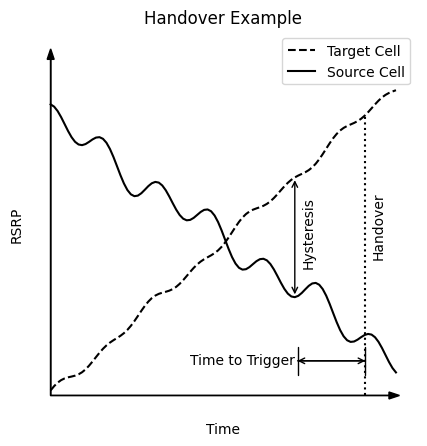
\includegraphics[width=0.48\textwidth]{src/img/hysteresis_ttt.png}}
    % 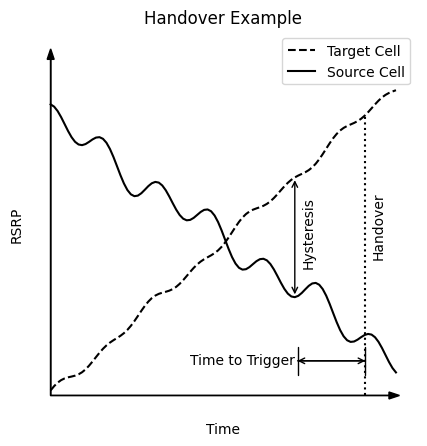
\includegraphics[width=0.48\textwidth]{src/img/hysteresis_ttt.png}
    \caption{handover based on Hysteresis and TTT}
    \label{fig:hysteresis_handover}
\end{wrapfigure}

The standard approach towards handover uses two parameters, \textit{Hysteresis} and \textit{Time to Trigger}, to determine when to trigger handover. When a neighbour cell has an RSRP greater than the current cell by a set margin, i.e. the Hysteresis, for a given period, i.e. time to trigger, the handover is triggered, and the UE is transferred to the neighbour cell. This process is illustrated in Figure \ref{fig:hysteresis_handover}. Alternative heuristics are often needed, as the standard approach is not robust enough for dynamic environments.



\clearpage %============================= CLEAR PAGE  =====================================%

\subsection{Alternative Heuristics}
The majority of existing handover algorithms use relative RSRPs (such as Hysteresis) with some delay (such as Time to Trigger). Other parameters suggested and modelled in the literature are throughput, location, load balancing, user velocity, service delay, and distance. \cite{nyangaresi_efficient_2022}.

\citet{hatipoglu_handover-based_2020} presented a handover-based load balancing algorithm for HetNets. The paper utilised UE speeds in determining handover, which is an unrealistic metric to obtain in practice. The algorithm itself is pretty simplistic, and while the paper showed promising results, the algorithm does not consider critical metrics such as RSRP or connection speed.

\subsection{Machine Learning}
Seeing handover as an optimisation problem, using machine learning (ML) to solve the handover problem is natural. For this reason, ML techniques are appealing to provide better performance than the more naive algorithms. As ML techniques do not require a model of the environment, this is especially applicable to indoor environments, where modelling proves difficult.

ML algorithms can be subdivided into supervised, unsupervised and reinforcement learning. Supervised and unsupervised algorithms perform regression or classification on a set of inputs. Reinforcement learning is based on the idea that the algorithm will learn to maximise its rewards in a given environment by learning the optimal policy. In our case, the optimal policy is a sequence of handover decisions that maximise throughput while minimising HOF and HOPP. The use of reinforcement learning has been surveyed in \cite{mollel_survey_2021}.

Reinforcement learning is a broad grouping of algorithms. These include Multi-Armed Bandits, Monte Carlo methods, and Deep Q-learning.

\citet{yajnanarayana_5g_2020} presented a handover algorithm using Contextual Multi-Armed Bandit reinforcement learning. This ML model provided modest improvements (0.3dB) in the average RSRP of devices. The authors also built their custom network simulator, which used sophisticated propagation models like log-shadowing and the WINNER UMa Model. The code used to simulate it was not released, providing very little reproducibility of the paper. The improvements were relatively minor, and better results could be obtained with a deep-learning-based Reinforcement model.

\citet{mollel_survey_2021} further introduces and surveys an alternative machine learning method. The pure network-based models operate only on radio data, such as RSRP and base station states. However, an alternative heuristic uses optical information, such as camera feeds, to predict handover better. This is done by tracking UE movement through object detection and predicting when LOS will be obstructed. While this tool can prove very useful, it introduces many limitations, as the models trained will be very location-dependent and have the most significant impact in indoor environments due to the greater LOS blockage rate.

\section{Handover Testbeds}
To evaluate experimental algorithms, we need some way to emulate a network. Many authors run custom simulations using propagation algorithms to model path loss and simulate the network devices. A better method is using a software radio suite as a testbed. This allows us to emulate UEs, base stations (BSs), and the core network (CN).

A few options are available, with the major software being srsRAN, OpenAirInterface, and Aether. This paper chose srsRAN due to its clear open-source code and extensive tutorials. While a fully custom testbed allows for greater flexibility, the realistic nature of using software radio suites will give results that much better reflect how the algorithms would perform in a real-world scenario and, so, arguably, give more useful results.

\citet{powell_handover_2021} presented a testing framework for 4G experiments using srsRAN and performed basic experiments. The framework was presented clearly, and I was able to replicate the results of their simulation. The experiments they performed, however, were limited as signal strength was arbitrarily introduced by attenuating a signal and did not utilise signal propagation algorithms.

% 3.5 pages, need to expand to maybe 7?

\section{Previous Work}
\tocomplete{Expand previous work}
\begin{itemize}
    \item \url{https://eudl.eu/pdf/10.1007/978-3-030-05195-2_39}
    \item \url{https://www.researchgate.net/publication/356947198_Evaluating_Handover_Performance_for_End-to-End_LTE_Networks_with_OpenAirInterface}
    \item \url{https://indjst.org/download-article.php?Article_Unique_Id=INDJST2579&Full_Text_Pdf_Download=True}
    \item \url{https://dl.acm.org/doi/pdf/10.5555/3466184.3466549}
    \item \url{https://arxiv.org/pdf/2307.14152.pdf}
    \item \url{https://ieeexplore.ieee.org/stamp/stamp.jsp?tp=&arnumber=6214116&tag=1}
\end{itemize}

\section{Further Technologies}
When examining the directions for this paper, three possible technologies should be reviewed as they strongly relate to either handover performance or experimentation. 

\subsection{Reactive vs Predictive Handover}
There are two main strategies when dealing with handover. We can either react to degraded quality and handover to improve it, or we can predict when quality is about to degrade and handover to maintain the quality of the connection.

\subsubsection*{Reactive Handover} This is the traditional handover mechanism where the decision to switch from one cell to another is made based on current signal strength and quality. This relies on a more static environment where no sudden drops in signal connection occur, as if a connection falls below a certain threshold, the cell cannot communicate the degraded connection to the eNB base station and must perform a reconnection to the network -- a Handover Failure. This also relies on real-time signal metrics, as a delayed response to a falling signal strength could result in a Handover Failure. While drawbacks exist when there is not a long enough window to react in, it is a much simpler algorithm to implement, and so is chosen for the majority of outdoor handover scenarios, with the exception of high-speed movement applications such as railways \cite{Kosmopoulos2022Handover} as well as other dynamic environments.
                
\subsubsection*{Predictive Handover} Predictive handover instead attempts to predict when signal quality is about to drop and initiates handover before the signal quality drops below a certain threshold. It aims to minimize disruption and enhance the user experience by anticipating network conditions \cite{Al-Quraan2023Enhancing}. This avoids Handover Failures as seen in Reactive Handovers but relies on accurate predictions. Prediction misses could instead lead to a much larger amount of unnecessary handovers, some of which may be classified as Ping Pong Handovers.  Many Predictive Handovers utilise UE movement speed to estimate when to initiate a handover. However, many now leverage machine learning algorithms to predict the need for handover. This requires accurate historical data and real-time analysis for prediction, and signal processing techniques are incorporated to analyze patterns and predict future signal degradation.

\subsubsection*{This Paper} While we aim to initially examine the performance of reactive handovers in indoor environments, we wish to examine the feasibility of introducing a Predictive Handover algorithm, however this may be beyond the scope of this paper, and so we instead lay the groundwork for future research in this area.

\subsection{Large Scale Emulators}
We can fully simulate network environments in software; however, this is limited in its ability to extract useful insights for new environments. There is an alternative, however, in the form of large-scale network emulators, the largest of which are the Platforms for Advanced Wireless Research (PAWR). These do not rely on software simulation but consist of real-world software-defined radio testbeds. Specifically, their POWDER platform is a city-wide testbed in Utah in the United States. 

POWDER allows researchers to run experiments without maintaining and deploying networks themselves. This removes many barriers to entry in the research of 4G/5G networks, as the costs of equipment can be fairly high. It also enables researchers to test machine learning models for predictive handover and assess signal processing algorithms in a controlled environment.   \cite{Rusca2023MobileRF}.

For this paper, POWDER was not used as the group already had a working testbed; however, this remains a viable route for larger-scale experiments for an extension to this project. Furthermore, while the scale of POWDER is very large, provision for indoor handover scenarios is not very high.

\subsection{O-RAN}
Open Radio Access Network (O-RAN) architecture is a new standard of network organisation that promotes interoperability and flexibility in 5G networks. It defines standardised interfaces (E2) for modular radio network components to communicate over and includes the RAN Intelligent Controller (RIC), a software-defined component responsible for controlling and optimising RAN functions [https://www.juniper.net/gb/en/research-topics/what-is-ric.html]. \todo{extract this into citation}

This enables the integration of machine learning directly into the radio access network for smarter handover decisions and innovation and customization in handover strategies by allowing third-party applications and services within the RAN  \cite{Niknam2020IntelligentORAN}. 
\todo{clean up this section, and make it relatable to the rest of the paper}

\tocomplete{Mention CQI in this section}
\tocomplete{Mention Hard vs Soft Handover}

% \bibitem{Rusca2023MobileRF}
% R. Rusca, F. Raviglione, C. Casetti, P. Giaccone, F. Restuccia, "Mobile RF Scenario Design for Massive-Scale Wireless Channel Emulators," \emph{2023 Joint European Conference on Networks and Communications \& 6G Summit (EuCNC/6G Summit)}, 2023.

% \bibitem{Niknam2020IntelligentORAN}
% S. Niknam, A. Roy, H. S. Dhillon, S. Singh, R. Banerji, J. H. Reed, N. Saxena, S. Yoon, "Intelligent O-RAN for Beyond 5G and 6G Wireless Networks," \emph{2022 IEEE Globecom Workshops (GC Wkshps)}, 2020.


% \bibitem{Kosmopoulos2022Handover}
% I. Kosmopoulos, E. Skondras, A. Michalas, E. T. Michailidis, D. Vergados, "Handover Management in 5G Vehicular Networks," \emph{Future Internet}, vol. 14, no. 2, 2022. Available: https://doi.org/10.3390/fi14020049

% \bibitem{Al-Quraan2023Enhancing}
% M. M. Al-Quraan, A. Zoha, A. Centeno, H. Salameh, S. Muhaidat, M. Imran, L. S. Mohjazi, "Enhancing Reliability in Federated mmWave Networks: A Practical and Scalable Solution using Radar-Aided Dynamic Blockage Recognition," \emph{arXiv.org}, 2023. Available: https://arxiv.org/abs/2301.05496



\chapter{Exploratory Research Design}
\label{chap:exploratoryResearchDesign}

\section{Overview of Approach}
Due to the iterative nature of exploratory work, this paper is not structured by methodology, results, and discussion but progresses iteratively. For our results to be meaningful and to progress in an efficient manner, the research of the paper is structured into multiple experimentation cycles. Each cycle is comprised of:

\begin{enumerate}
    \item Determining Objective(s)
    \item Defining Hypotheses
    \item Build Approach
    \item Present Results
    \item Immediate Discussion
\end{enumerate}

This structure allows for a more flexible approach to the research. It allows us to adapt as new insights are gained and form new hypotheses without compromising the experiment. This supports the dynamic nature of exploratory research, where learning and adaptation are key.

\subsection*{Determining Objective(s)}
The first step in each experimentation cycle is to clearly define what objective we are trying to achieve. This objective, or objectives, guide the research for the cycle, determining which hypotheses are chosen and how to approach the research. Objectives may be refined or adjusted as data is gathered and new insights are formed.

\subsection*{Defining Hypotheses}
As objectives are chosen, we can begin formulating hypotheses we aim to test or explore. We will test these predictions and provide a clear direction for the experimentation and analysis phases. Hypotheses should be specific and should not change as new data is gathered -- for that, we can note down the new questions that arise, which will inform the next research cycle.

\subsection*{Build Approach}
With our objectives and hypotheses defined, this stage will focus on designing and planning our experimentation process. This includes selecting methodologies, defining which data to collect and how, and outlining the analysis techniques to be employed. This approach should be designed to efficiently test and answer the stated hypotheses, achieving the cycle's objectives.

\subsection*{Present Results}
This section presents all results from the experimentation and analysis of said data. The results should be detailed for clear analysis and focused on transparency and reproducibility to support the next discussion phase and future research.

\subsection*{Immediate Discussion}
This final phase is an immediate critical discussion of the derived results. The data provides insights and discusses the implications for the paper's wider research goals. These insights and results feed directly into the design of the next cycle, and the learning gained, in turn, informs how we structure the following objective and approach.


\section{Initial Hypotheses}
We wish to test four main hypotheses in this paper. We discuss the reason for their inclusion, what proving the hypotheses means regarding our research goals, and what contradicting them would indicate.

\subsection{Ping Pong Handover Prevalence}
Ping Pong Handover will be much more prevalent due to the denser configuration of indoor networks.
\begin{itemize}
    \item \textbf{Expectation:} Increased Ping Pong Handovers are anticipated due to the closer proximity of access points and the resulting signal overlap. Small signal fluctuations could result in a handover to a neighbour cell and then immediately back again.
    \item \textbf{Implication:} A higher incidence of Ping Pong Handovers could indicate a need for more careful tuning of handover parameters or even more sophisticated handover algorithms tailored to dense environments - such as a Machine Learning based one.
    \item \textbf{Consideration:} Contradicting this hypothesis may suggest existing handover mechanisms are more effective in dense configurations than anticipated or that signal management techniques are mitigating expected issues.
\end{itemize}

\subsection{RSRP Stability}
RSRP values will be less stable due to a more dynamic environment induced by the movement of persons and greater signal reflection from walls, doors, and obstacles.
\begin{itemize}
    \item \textbf{Expectation:} Fluctuations in RSRP (Reference Signal Received Power) greater than expected (see \insertref) due to the aforementioned reasons. We expect these to arise from the more constrained environment providing greater signal reflection and the higher likelihood of LOS blockage due to the lower relative transmitter height.
    \item \textbf{Implication:} Unstable RSRP values may necessitate adjustments in network planning and signal optimization strategies to ensure consistent user experience. Care must be taken regarding possibly dampening signal gain.
    \item \textbf{Consideration:} If RSRP values are found to be more stable than expected, it could point towards an inherent robustness in the network's design against indoor environmental variables. Signal reflections could be overstated, and LOS blockage may not play a large role in lower-frequency transmission.
\end{itemize}

\subsection{Unnecessary Handovers}
The number of unnecessary handovers will be very high - independent of the change in CQI and level of throughput. Unnecessary handovers are defined as those that do not improve user experience and partially overlap with the Ping Pong metric.
\begin{itemize}
    \item \textbf{Expectation:} A significant volume of handovers may occur without corresponding benefits regarding improved signal quality or throughput, indicating inefficiencies in the handover process.
    \item \textbf{Implication:} High rates of unnecessary handovers could lead to network resource wastage and degraded user experiences, highlighting areas for optimization.
    \item \textbf{Consideration:} Should this hypothesis be contradicted, it might reveal that current handover criteria are more effective than predicted at minimizing unnecessary transitions.
\end{itemize}

\subsection{Impact on Total Throughput}
The total throughput will be lowered as a result of the frequent handovers.
\begin{itemize}
    \item \textbf{Expectation:} Frequent handovers are presumed to disrupt data flows, thereby reducing the overall network throughput.
    \item \textbf{Implication:} A drop in throughput due to handovers suggests a need for balancing handover triggers with throughput preservation, possibly by refining handover algorithms.
    \item \textbf{Consideration:} If throughput is not adversely affected by handover frequency as hypothesized, it could indicate that the network efficiently manages handovers to minimize the impact on data transmission.
\end{itemize}


\section{Research Lab Layout}
The testbed used to run many of the experiments is set up in one of the labs used by the Edinburgh NetSys Group. It consists of a node cluster which hosts the network core, and 4 Intel NUCs \insertref, each connected to an Ettus Research B210 USRP \insertref, which acts as the base stations. These USRPs are Software Defined Radios; this allows a network simulator to use them to send and receive radio signals with arbitrary coding schemes and frequencies, a key requirement for development and research testing.

Below is a top-down view of the testbed used by the Edinburgh NetSys Group. Units are in centimetres, and the boxes with a cross through them represent the locations of the B210 USRPs. The door is on the left-hand side. The USRPs on the top of the image are on a shelf 127cm above the ground, and the 2 USRPs on the bottom of the image are on a desk 80cm above the ground.

\begin{figure}[!h]
    \centering
    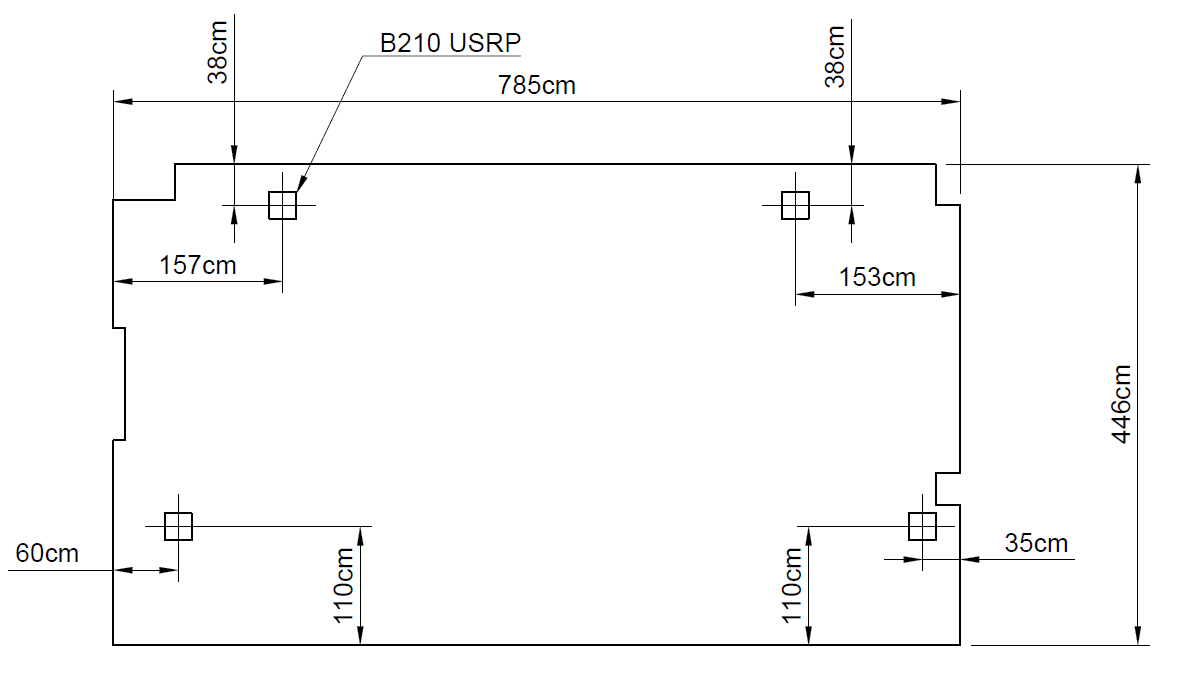
\includegraphics[width=1\linewidth]{src//img/room117tesbed.png}
    \caption{Radio Testbed Layout}
    \label{fig:appendix:testbed-drawing}
\end{figure}

\section{Software Stack}
There are multiple software artefacts needed to run the testbed. To run the base stations, srsRAN's eNB code is used to control the USRPs that host the radio layer of the network. For (\todo{add reasons}), we use open5gs to run the network core, which is responsible for authenticating users, orchestrating the network and providing a control flow. A Kubernetes \insertref deployment is used to run all of these simultaneously, nominating the base stations and core network as pods and the physical NUCs and clusters as the nodes. The exact tools were used with generous permission from Jon Larrea [https://orcid.org/0000-0001-5736-2107], the author of the deployment tools.

\todo{Add a figure here maybe?}

\section{UE setup}
\tocomplete{Finish UE setup}
\begin{itemize}
    \item The phone
    \item The laptop
\end{itemize}


\chapter{Experimentation}

\textcolor{orange}{we need a paragraph here to briefly explain the experimentation section, what we do here}

\section{ZMQ-based Handover in srsRAN}
\subsection{Objective}
The first phase aims to understand the basics of S1 handover \textcolor{orange}{or we explain what is S1 we assume that it is just handover without the S1} using srsRAN in a controlled simulation. We can use ZMQ and GNU radio to emulate the radio layer. \textcolor{orange}{cite ZMQ and GNU radio? Explain a bit what they are}

\subsection{Approach}

\textcolor{orange}{several bullet points do not have the dot that ends the sentence}

\begin{itemize}
    \item Following \cite{powell_handover_2021}, I started with a pure simulation-based experiment of inducing an S1 handover
    \item This is accomplished by using ZMQ and GNU Radio to simulate the radio layer.
    \item We set up the experiment by running an Open5gs network core, two srsENBs and a srsUE \textcolor{orange}{describe what is srsENB and srsUE}
    \item The eNBs are connected to the network core over the S1AP interface over TCP on my local machine
    \item The eNBs were both connected to the UE using GNU radio and ZMQ, communicating over various TCP ports.
    \item To emulate propagation loss, we add `multiply` blocks on both connections (send and receive) from UE to each eNB, initially setting it to 1 for the eNB we designate as the source cell and 0 for the "target" cell \todo{insert screenshot of GNU flow graph}
    \item On the srsUE process, we collect the measurement logs, fetching the RSRP for both cells
    \item We gradually increase the multiply for the target cell, until the UE is handed over to the target cell
\end{itemize}

\subsection{Results}
\begin{itemize}
    \item Figure \ref{fig:methods:zmq-s1-handover} shows the results of said experiment
    \item As the handover is triggered by default using the A3 Event Trigger, we can see that the A3 offset used in our configuration was 3dBm.
    \item On a static source analysis of the srsRAN code we see the handover occurs when the following condition is met:
$$\text{RSRP}_\text{Target} - \text{RSRP}_\text{Source} > \text{Hysteresis} + \text{A3 Offset} + \text{Of} + \text{Oc}$$
where 
$$\begin{aligned}\text{Of} &= \text{Frequency Offset}_\text{Target} - \text{Frequency Offset}_\text{Source} \\
\text{Oc} &= \text{Cell Offset}_\text{Target} - \text{Cell Offset}_\text{Source}\end{aligned}$$
for the default setup, $\text{Of}=0$ and $\text{Oc}=0$
\item Furthermore, Hysteresis is set to 0, and in our configuration, A3 Offset was set to 3dBm, so we see srsRAN behaving as expected according to the LTE specification.
\end{itemize}
\begin{figure}
    \centering
    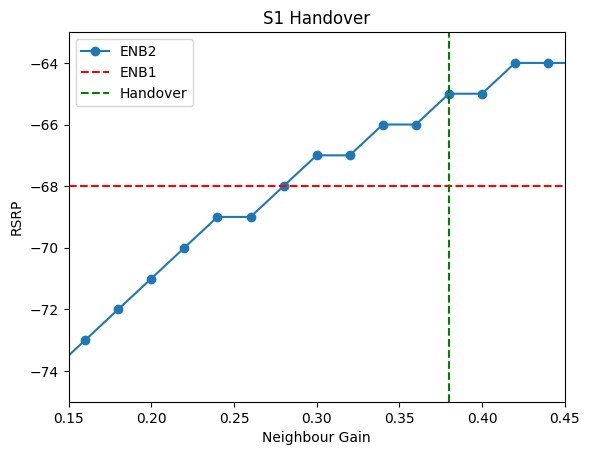
\includegraphics[width=1\linewidth]{src/img/zmq_s1_handover.png}
    \caption{S1 Handover occurring in srsRAN with simulated UE over ZMQ/GNU Radio}
    \label{fig:methods:zmq-s1-handover}
\end{figure}
\subsection{Immediate Discussion}
This phase confirmed srsRAN's adherence to the LTE standard, and a handover was successfully performed in a simulated environment. This phase was limited by the simplistic nature of the simulated radio network, as constants purely dictated network strength. The limited nature of the simulated environment prompted questions about how handovers would occur in more complex environments.

\section{Custom Network Simulator for Large Scale Handovers}
\label{sec:exp:custom}
\subsection{Objective}
Building on the initial findings, this phase was focused on understanding the ping-pong metric and the associated triggers, employing a custom large-scale simulator for analysis.

\subsection{Approach}
Inspired by \citep{hatipoglu_handover-based_2020}, we reconstructed their non-disclosed tool to simulate large-scale handovers.
\begin{itemize}
    \item We look at  to better understand how large-scale handovers are conducted
    \item We replicate their findings to understand what causes ping-pong
    \item Propagation loss was modelled with path shadow loss (insert equations here) \textcolor{orange}{YOU NEED TO DO IT}
    \item UE movement is simulated using a random walk with various speed categories
    \item As the authors did not release the tool they built, we reconstructed the tool, as seen in Figure \ref{fig:methods:grouped-uesim} \textcolor{orange}{explain the figure correctly, what are the axis? What do the colors mean?}
\end{itemize}
\begin{figure}
    \centering
    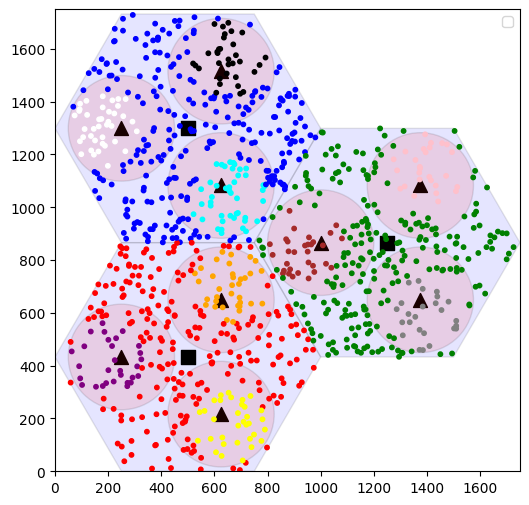
\includegraphics[width=0.75\linewidth]{src//img/grouped_uesim.png}
    \caption{An overview of the 2D simulator}
    \label{fig:methods:grouped-uesim}
\end{figure}
\subsection{Results}
We run the experiment with various handover parameters in Figure \ref{fig:methods:pingpong-uesim}. The impact of the hysteresis value becomes apparent \todo{redo graph showing z-axis} \textcolor{orange}{I miss an explanation of figure 4.3 and the insight of this experiment. Is TTT T(time to trigger) defined somewhere?}
\begin{figure}
    \centering
    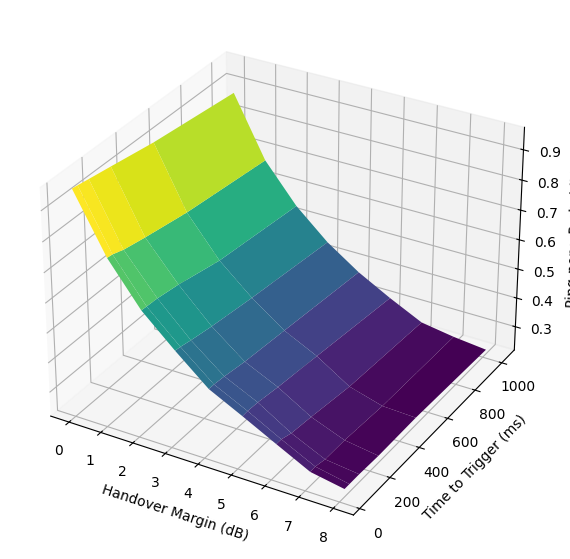
\includegraphics[width=0.5\linewidth]{src//img/pingpong_uesim.png}
    \caption{Ping Pong vs Hysteresis and TTT}
    \label{fig:methods:pingpong-uesim}
\end{figure}
\subsection{Immediate Discussion}
The simulator offered some insights into the conditions that cause ping-pong handovers; however, this was majorly limited by the basic nature of the loss propagation function and highly approximate human movement. This once again reiterates the need for real-world testing to validate these findings \todo{do we validate?}, leading to our next phase of experimentation.


\section{Real-world Network Testbed Implementation}

\subsection{Objective}
After performing the initial experiments in a simulator, we move on to testing in the real world to validate our simulation insights and provide real insight into indoor scenarios. We use a network of radio-enabled srsENBs to examine handover behaviour in a physical environment.

\subsection{Approach}
We plan on performing a range of experiments using the setup described in Sections \ref{sec:research-lab-layout} and \ref{sec:research-software-stack}. These experiments are outlined in the following subsections.

\subsection{Mobility Tests}
\label{sec:exp:real:mobile}
\subsubsection{Objective}
We wish to examine the performance of the indoor handover in various mobility settings.
\subsubsection{Approach}
To reduce confounding variables, we start the network with only two eNBs for this experiment. We examine four different mobility settings:
\begin{itemize}
    \item[\textbf{Stationary}] We set up this experiment by placing the UE machine between the two eNBs and taking care of the environment remaining entirely static; the UE remained stationary, and no persons moved during the experiment. Here, we expect no handover will occur and that the radio signal (as measured by RSRP) will remain constant.
    \item[\textbf{Walking}] We set up this experiment by initially starting the data recording when the UE is near one eNB and then walking towards the other side of the room with the second eNB. Once we reach the eNB, we return to our initial position. To eliminate external factors, no other person was in the lab, and the movement speed was kept roughly constant. We expect the signal strength of the UEs \textcolor{orange}{are we using one UE? Or more?} to vary proportionally to the distance we are from them and expect a handover to occur once we have moved beyond halfway between the UEs. We expect a second handover on the way back.
    \item[\textbf{Rotating}] This experiment was devised to determine the impact of the angle of UE on the corresponding signal strength. We enable two eNBs on the same wall and place the UE halfway between the eNBs in the centre of the room. We slowly rotate the USRP between the two eNBs, back and forth. We expect no significant change in the signal quality, as LOS is not lost, and the distance between the UE and eNBs does not change.
    \item[\textbf{Dynamic Environment}] In this experiment, we aim to test the network's response to a more dynamic environment. The UE is placed in the same position as the \textbf{Rotating} experiment, facing towards the eNBs' midpoint. During the experiment, a person walks in front of the UE and back again, simulating people walking around in a room. We expect some small drop in the signal strength as LOS with the corresponding eNBs is lost, but we believe that signal reflections contribute a sufficient proportion of the signal strength.
\end{itemize}
\subsubsection{Results}
The real-world experiments and the description of the experiment are set out in Figure \ref{fig:methods:real-world-testbed}. \textcolor{orange}{explain further the general idea of the figure. Color represents that the UE is connected to an eNB, if the color changes this means that the UE is associated with another eNBs. Could you also increase the font size of the axis?}
\begin{figure}[p]
    \centering
    \caption{Real-world Network Testbed Implementation: A series of experiments illustrating various aspects of handover behaviour in a real-world setup.}
    \label{fig:methods:real-world-testbed}
    \begin{minipage}{0.45\textwidth}
    \begin{subfigure}{\linewidth}
        \centering
        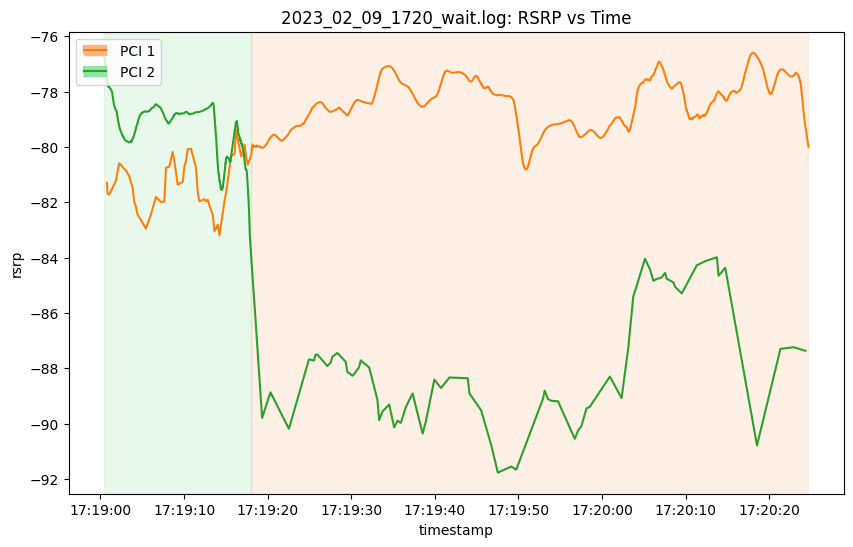
\includegraphics[width=0.9\linewidth]{src//img/2024_02_09_wait.png}
        \caption{Stationary}
        \label{fig:real:mobile:wait}
    \end{subfigure}
    \end{minipage}
    \begin{minipage}{0.45\textwidth}
        \small{Figure \ref{fig:real:mobile:wait}: Shows the effect of no movement on RSRP measurements, indicating the presence of environmental noise and its potential impact on handover decisions.}
    \end{minipage}
    
    \vspace{1cm}
    \begin{minipage}{0.45\textwidth}
    \begin{subfigure}{.9\linewidth}
        \centering
        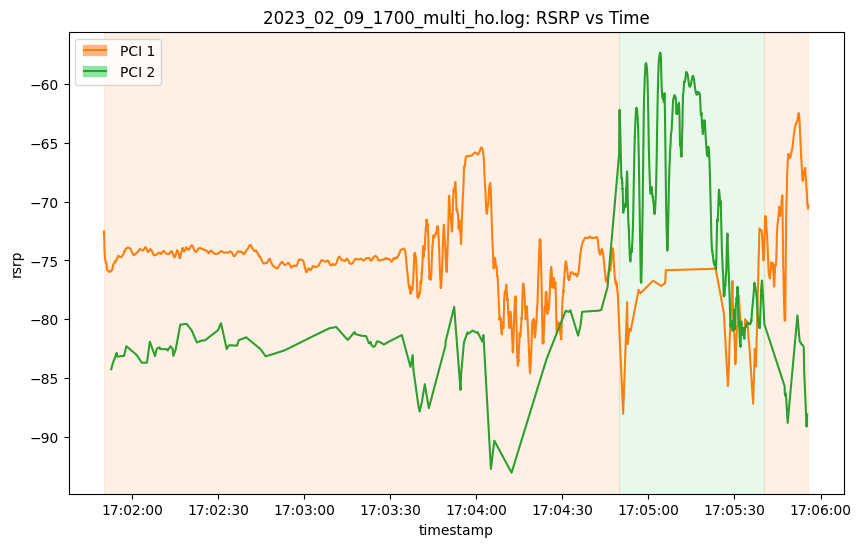
\includegraphics[width=0.9\linewidth]{src//img/2024_02_09_multiho.png}
        \caption{Walking back and forth}
        \label{fig:real:mobile:walk}
    \end{subfigure}
    \end{minipage}%
    \begin{minipage}{0.45\textwidth}
        \small{Figure \ref{fig:real:mobile:walk}: Demonstrates the RSRP and connected cell for a walking back and forth episode. This experiment showcases the dynamic RSRP changes as the UE moves closer or further from each eNB.}
    \end{minipage}
    
    \vspace{1cm}
    \begin{minipage}{0.45\textwidth}
    \begin{subfigure}{\linewidth}
        \centering
        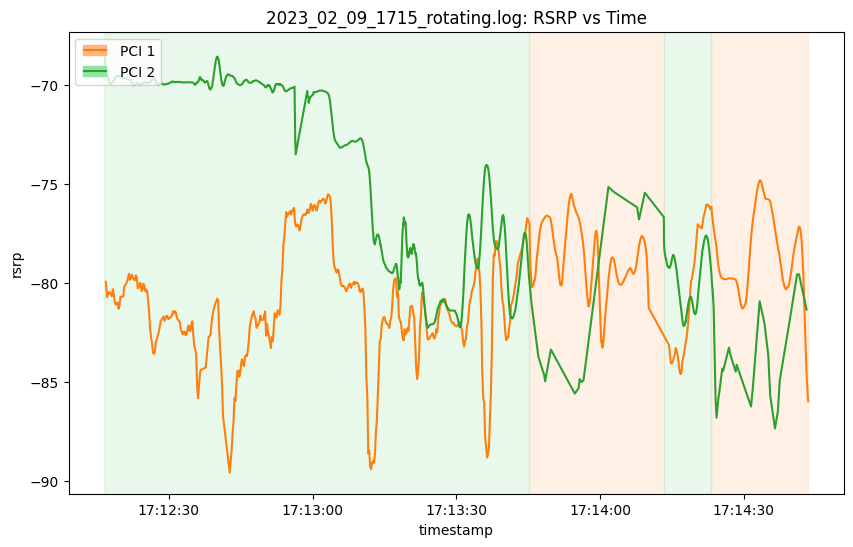
\includegraphics[width=0.9\linewidth]{src//img/2024_02_09_rotating.png}
        \caption{Rotating UE}
        \label{fig:real:mobile:rotate}
    \end{subfigure}
    \end{minipage}
    \begin{minipage}{0.45\textwidth}
        \small{Figure \ref{fig:real:mobile:rotate}: Illustrates the impact of rotating the UE on RSRP fluctuations and handover events, highlighting the sensitivity of handover mechanisms to device orientation.}
    \end{minipage}
    
    \vspace{1cm}
    \begin{minipage}{0.45\textwidth}
    \begin{subfigure}{\linewidth}
        \centering
        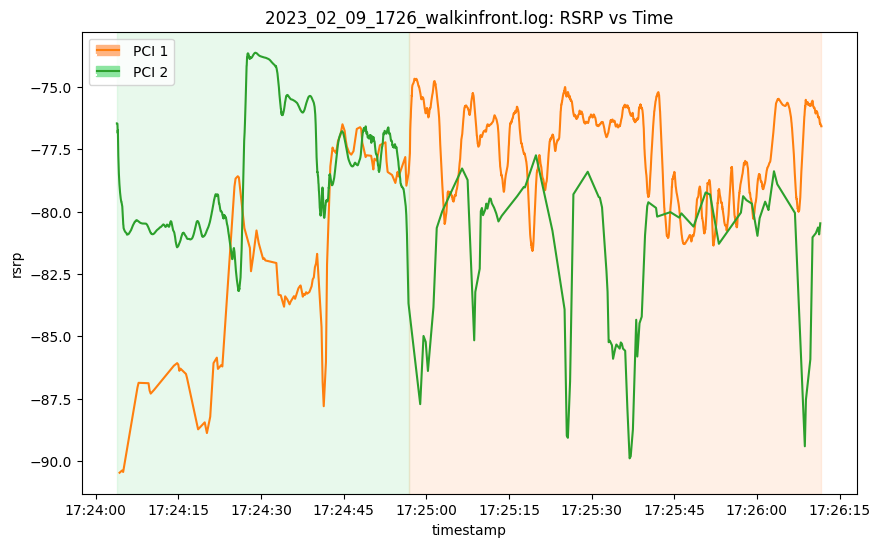
\includegraphics[width=0.9\linewidth]{src//img/2024_02_09_los_block.png}
        \caption{LOS Blockage by walking around}
        \label{fig:real:mobile:block}
    \end{subfigure}
    \end{minipage}
    \begin{minipage}{0.45\textwidth}
        \small{Figure \ref{fig:real:mobile:block}: Examines the effects of line-of-sight (LOS) blockage by simulating movement around the UE. This scenario reflects real-world dynamics where human movement can influence signal quality and handover behaviour.}
    \end{minipage}
\end{figure}
\subsubsection{Immediate Discussion}
These findings underscored the complexity of indoor scenarios.

Figure \ref{fig:real:mobile:wait} shows the high impact of environmental noise even in stationary situations \textcolor{orange}{explain it more we expected no change on the RSRP but is not the case. We observe that even in stationary environments, there is a big change in the RSRP, and this triggers handover. Explain why this is happening, any interesting finding is appreciated, we need to show the reader anything relevant}. Figure \ref{fig:real:mobile:walk} performs handovers as a UE moves closer and further from a target cell as expected \textcolor{orange}{Explain it further, the UE moves linearly between the eNBs, we expect the RSRP to behave in this way (the RSRP does it? It seems that RSRP does not change smoothly). There is a handover once the UE approaches the second eNBs and another once it gets further. }. However, the large noise spikes were not accounted for in the expectations of the experiment. The following experiment in Figure \ref{fig:real:mobile:rotate} seeks to highlight this possible disparity by rotating the UE back and forth, causing significant disturbances to RSRP \textcolor{orange}{explain it further, why do we have 3 handovers? Does this make sense? Please talk about the figure and provide some insight if possible}. Finally, Figure \ref{fig:real:mobile:block} highlights further issues caused by the dynamic environment \textcolor{orange}{the same with this figure}.

The four experiments together highlight the high difficulty of indoor handover. \textcolor{orange}{Talk more of the general idea, the RSRP changes quickly and it does not behave as expected. This challenges indoor handover. You need to provide more details}

\subsection{Handover Impact on Latency}
\label{sec:handover-impact}
\subsubsection{Objective}
To understand the level of the issues found in the previous experiment must be mitigated, through which unnecessary handovers are reduced, we must understand the impact on metrics such as throughput and latency of the connection. This experiment focuses on the latency introduced by an individual handover.

\subsubsection{Approach}
To determine the latency impact of a handover event, we utilise ICMP \texttt{ping} messages. We setup the UE to have ping messages sent to the EPC every 10ms. We simultaneously use \texttt{tcpdump}\insertref to capture all incoming and outgoing packets. We then can use Wireshark\insertref to analyse the return trip time (RTT). We use Wireshark's inbuild graphing tool to produce a time series of the maximum RTT.

% \begin{itemize}
%     \item To determine the actual impact of a handover, we must measure it quantitatively
%     \item We run a ping flood from the UE to the EPC and capture the packets using `tcpdump`
%     \item Similarly to the previous experiment, we walk from one eNB to another to induce handover
%     \item The packet traces are then analysed with Wireshark to see the latency of each packet. We perform a rolling max smoothing with a window size of 2ms.
%     \end{itemize}

To capture a handover event, we set up the experiment similarly to Section \ref{sec:exp:real:mobile}'s walking experiment, walking from one eNB to the other.
\subsubsection{Results}
The results are shown in Figure \ref{fig:methods:ping-handover}
\begin{figure}
    \centering
    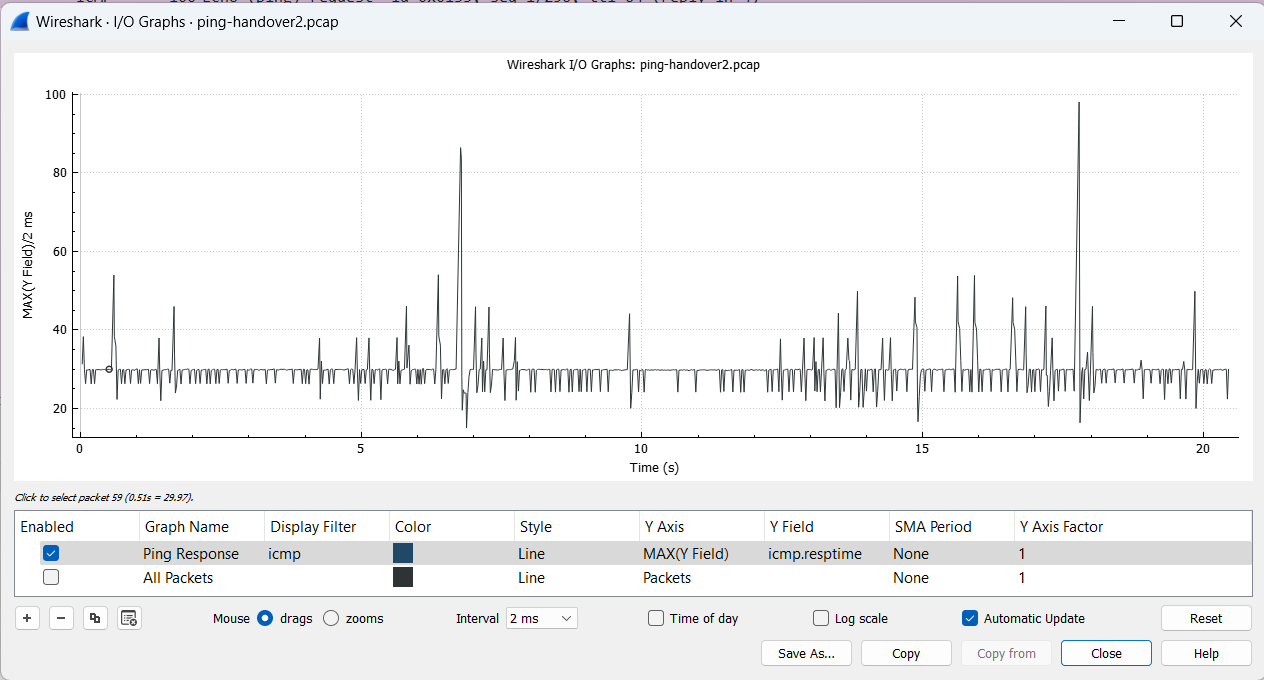
\includegraphics[width=0.75\linewidth]{src//img/ping-handover.png}
    \caption{Wireshark view of Ping during a handover event \textcolor{orange}{we need to make this figure bigger, y-axis is not well recognized}}
    \label{fig:methods:ping-handover}
\end{figure}
\subsubsection{Immediate Discussion}
We see a large latency spike during the handover event, however no packets are dropped due to the EPC/eNB buffering any packets received during HO. We can see that the latency maxes out at 96ms. This result is consistent with \citet{zhang_performance_2012}.

\subsection{Handover Impact on Throughput}

\textcolor{orange}{this subsection does not evaluate datarate for handover since the handover is not triggered in any of the two figures, 4.6 and 4.7. Raname by Throughput analysis in indoor environments?}

\subsubsection{Objective}
To further understand the impact of handover in indoor environments, we must also examine the throughput drop due to handover. This section focuses on repeating the mobility tests in Section \ref{sec:exp:real:mobile} while measuring throughput.

\subsubsection{Approach}
To measure the impact on throughput during a handover event, we must first determine an approach. We have two options in communication protocol: UDP and TCP. UDP, a best-effort protocol, contains no rate limiting or reliable message delivery; however, it can deliver the highest throughput. Conversely, TCP ensures reliable message delivery and varies the transmission bandwidth depending on packet loss. It also accounts for the majority of internet traffic. 

We can use the \texttt{iperf3} tool, a network performance tester, as it is the most popular software. It also allows both UDP and TCP testing.

\begin{itemize}
    \item We can set up the experiment by enabling all our eNBs and using our lab machine as a UE. We keep the environment and UE static during the experiment.
    \item We start an \texttt{iperf3} server on the EPC. Simultaneously, we begin a \texttt{tcpdump} process to capture all incoming packets
    \item For testing UDP throughput, we start a client on the UE in UDP mode. We set the bandwidth to 100Mbits/s to saturate the uplink.
    \item For TCP testing, we start the client in TCP mode. The bandwidth is automatically determined by the TCP protocol.
    \item We can then measure the throughput by examining the lengths of the incoming packets.
\end{itemize}
\subsubsection{Results}
Figure \ref{fig:4udp} shows a 30-second capture of UDP throughput. The RSRP values remain very constant however the throughput is very erratic. \textcolor{orange}{make figure bigger}

Figure \ref{fig:4tcp} shows 30 seconds of TCP throughput capture. The RSRP values are slightly different. However, the connected eNB has a higher signal strength than the UDP. The throughput is much more constant - due to the TCP rate limiting the connection. However, it transmits at a much lower rate than the UDP connection. Furthermore, there are connection failures lasting more than 2.5 seconds. \textcolor{orange}{any guess why this happens?}
\begin{figure}
    \centering
    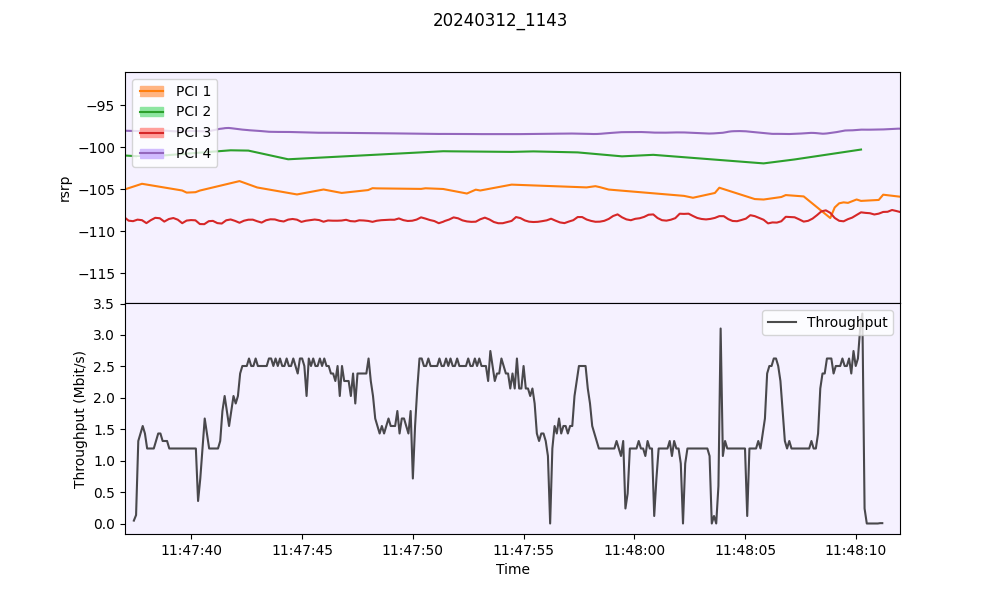
\includegraphics[width=0.5\linewidth]{src//img/4stationary_udp.png}
    \caption{Enter Caption}
    \label{fig:4udp}
\end{figure}
\begin{figure}
    \centering
    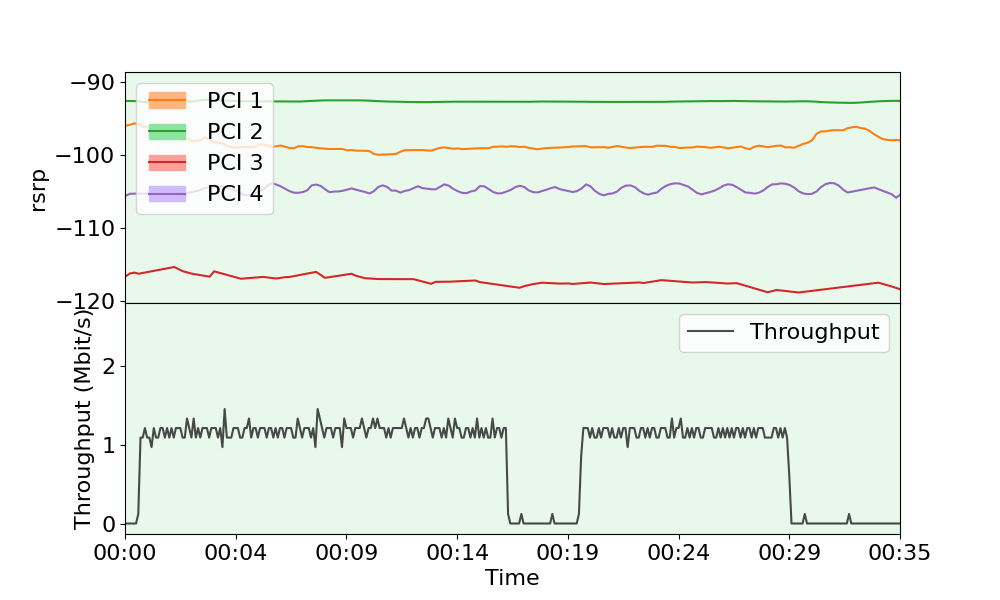
\includegraphics[width=0.5\linewidth]{src//img/4stationary_tcp.png}
    \caption{Enter Caption}
    \label{fig:4tcp}
\end{figure}

\subsubsection{Immediate Discussion}
Determining the best protocol to use for testing the network proves difficult. UDP provides a better understanding of the maximum throughput the connection can allow. However, TCP better emulates how regular communication affects the network.
Due to the network's inherent instability, TCP becomes a nonviable means of testing our network. As packet loss impacts TCP's communication ability, large gaps appear during our throughput measurements. This would limit our understanding of the effect of HO on throughput. Furthermore, we wish to test the network's maximum capacity, and so UDP provides a more granular view.

We, therefore, use UDP in our following experiments.

\subsection{Increasing cell density}
\tocomplete{}

\subsubsection{Objective}
The previous mobility tests were run with only two eNBs enabled. This is not representative of planned indoor deployments; instead, much higher cell density is expected \insertref \textcolor{orange}{that might be partially true, it will depend on the requirements}. This experiment focuses on the performance of the network with a higher number of active cells. We can hypothesise that with increasing cell density (more eNBs enabled) the rate of handover will be much higher.
\subsubsection{Approach}
We perform two sets of experiments, walking and stationary.
\begin{itemize}
    \item We start the experiment in the same way as the last. However, we enable all four eNBs.
    % \item We start a UDP iPerf3 server on the network core, and a client sending 100Mbits/s on the UE, to saturate the throughput
    % \item We capture incoming packets on the network core and use the volume of packets to measure throughput
    % \item We perform three experiments, a stationary one and two random walks through the lab.
    \item We smooth out the RSRP values with a moving average window of 1000ms% and the throughput values over 100ms.
\end{itemize}
\subsubsection{Results}
Results of the experiment are shown in Figures \ref{fig:real:4enb:stationary} and \ref{fig:real:4enb:walk}. \textcolor{orange}{I would not include Figure 4.8 since it is static and we do not have any handover while before we observed handover in static settings, so I would not include it. Please, explain Figure 4.9. The second subfigure seems to be longer and explains it. Explain the small handover, the handovers that last a few milliseconds.}

\begin{figure}
    \centering
    \includegraphics[width=0.75\linewidth]{src//img/4enbEx1Stationary.png}
    \caption{Stationary Capture of Thoughput}
    \label{fig:real:4enb:stationary}
\end{figure}
\begin{figure}
    \centering
    \caption{Moving Capture of Thoughput}
    \label{fig:real:4enb:walk}
    \begin{subfigure}{\linewidth}
        \centering
        \includegraphics[width=0.75\linewidth]{src//img/4enbEx2RandomWalk.png}
        \caption{Capture 1}
        \label{fig:real:4enb:walk1}
    \end{subfigure}
    \begin{subfigure}{\linewidth}
        \centering
        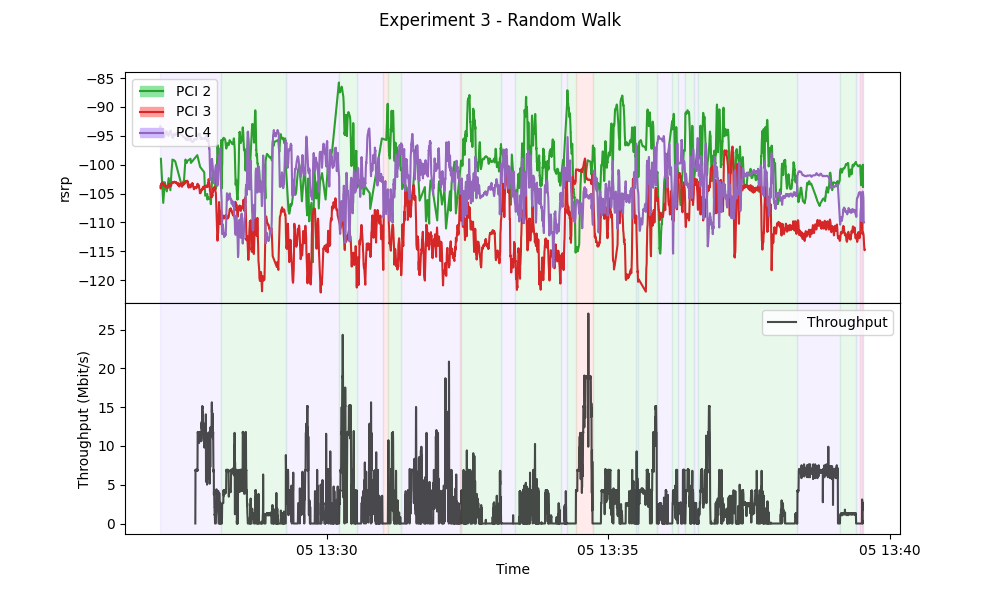
\includegraphics[width=0.75\linewidth]{src//img/4enbEx3RandomWalk.png}
        \caption{Capture 2}
        \label{fig:real:4enb:walk2}
    \end{subfigure}
    \begin{subfigure}{\linewidth}
        \centering
        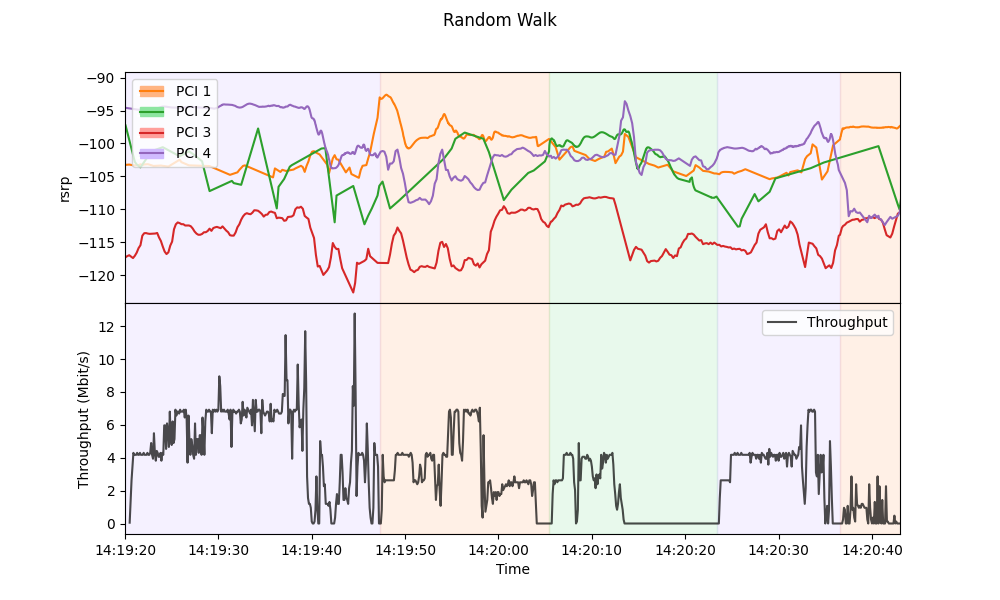
\includegraphics[width=0.75\linewidth]{src//img/4enbEx4RandomWalk.png}
        \caption{Capture 3}
        \label{fig:real:4enb:walk3}
    \end{subfigure}
\end{figure}

% \begin{figure}[p]
%     \centering
%     \caption{High Cell Density experiments: A series of experiments highlighting the increase HO-rate with more cells deployed}
%     \label{fig:real:4enb}
%     \begin{minipage}{0.45\textwidth}
%     \begin{subfigure}{\linewidth}
%         \centering
%         \includegraphics[width=0.9\linewidth]{src/img/4enbEx1Stationary.png}
%         \caption{Stationary}
%         \label{fig:real:4enb:stationary}
%     \end{subfigure}
%     \end{minipage}
%     \begin{minipage}{0.45\textwidth}
%         \small{Figure \ref{fig:real:4enb:wait}: Shows the effect of no movement on RSRP measurements. Against expectations, the signal remains fairly constant}
%     \end{minipage}
    
%     \vspace{1cm}
%     \begin{minipage}{0.45\textwidth}
%     \begin{subfigure}{.9\linewidth}
%         \centering
%         \includegraphics[width=0.9\linewidth]{src/img/4enbEx2RandomWalk.png}
%         \caption{Walking capture}
%         \label{fig:real:4enb:walk1}
%     \end{subfigure}
%     \end{minipage}%
%     \begin{minipage}{0.45\textwidth}
%         \small{Figure \ref{fig:real:4enb:walk1}: Of note, at 13:07:57, we see a ping pong handover that lasts only 57ms. Handover rate is 2.29 handovers/minute}
%     \end{minipage}
    
%     \vspace{1cm}
%     \begin{minipage}{0.45\textwidth}
%     \begin{subfigure}{\linewidth}
%         \centering
%         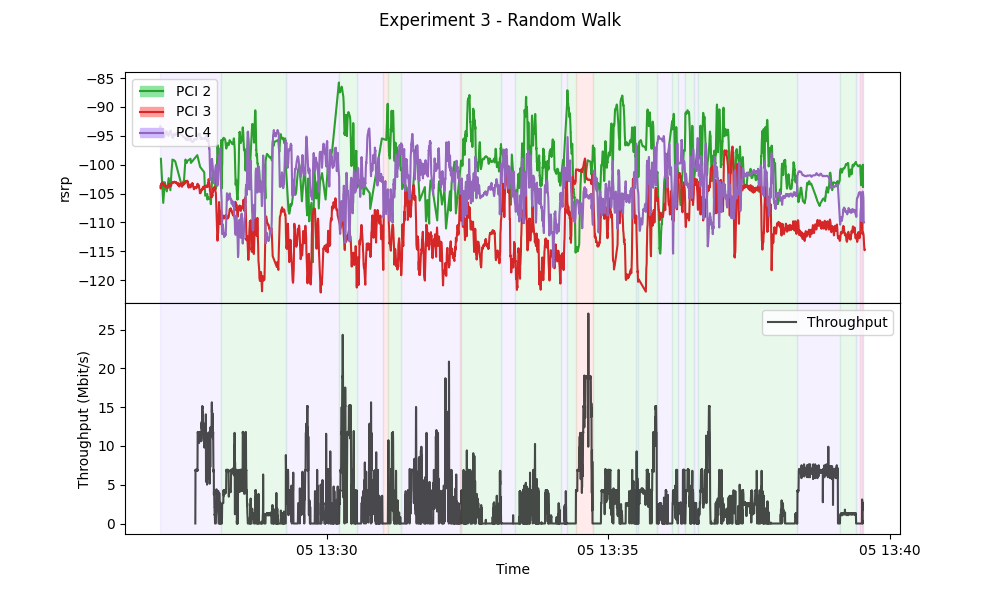
\includegraphics[width=0.9\linewidth]{src//img/4enbEx3RandomWalk.png}
%         \caption{Walking capture}
%         \label{fig:real:4enb:walk2}
%     \end{subfigure}
%     \end{minipage}
%     \begin{minipage}{0.45\textwidth}
%         \small{Figure \ref{fig:real:4enb:walk2}: Handover rate is 2.29 handovers/minute}
%     \end{minipage}
    
%     \vspace{1cm}
%     \begin{minipage}{0.45\textwidth}
%     \begin{subfigure}{\linewidth}
%         \centering
%         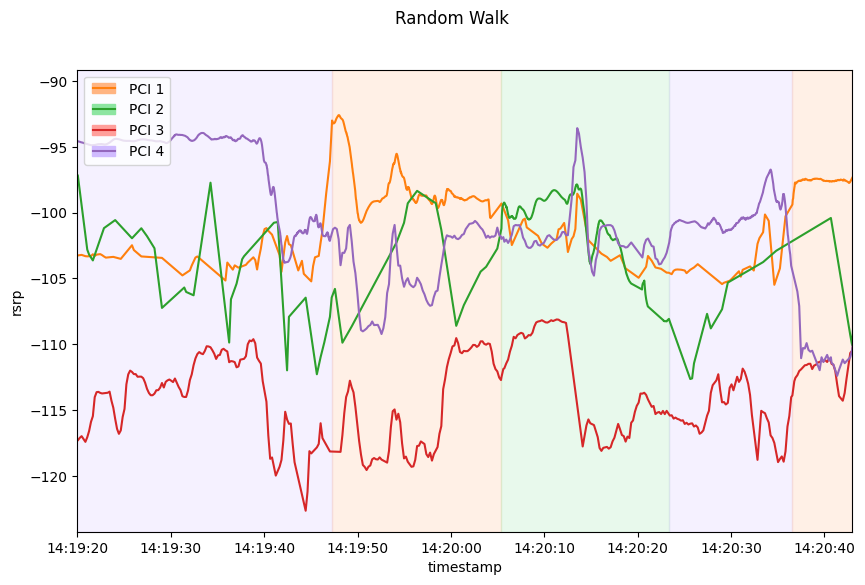
\includegraphics[width=0.9\linewidth]{src//img/real_4enb_walk3.png}
%         \caption{Walking capture}
%         \label{fig:real:4enb:walk3}
%     \end{subfigure}
%     \end{minipage}
%     \begin{minipage}{0.45\textwidth}
%         \small{Figure \ref{fig:real:4enb:walk3}: Handover rate is 2.89 handovers/minute}
%     \end{minipage}
% \end{figure}


\subsubsection{Immediate Discussion}
\begin{itemize}
    \item We see a high rate of handover, even when signal quality has not significantly fallen
    \item To properly understand, we must capture the throughput to see the impact of handovers.
    % \item For better analysis, we instead will attempt to use a TCP iperf3 server to utilise the more reliable protocol to control data flow.
    % \item Handovers occur fairly often, though, but none are under the 1-second threshold for ping pong handover.
    \item For the second walk, eNB with the PCI of 1, dropped off, a very common occurrence in the testing of the network - highlighting the difficulties of maintaining a network
\end{itemize}


% ===========================End Varying Cell Density================================ %



\subsection{Hysteresis Impact}
\tocomplete{}
\subsubsection{Objective}
During the previous experiments, we saw a very high rate of handovers, even when throughput was not improved. We turn to our tuneable parameters of handover, TTT and hysteresis. Considering our results in Experiment \label{sec:exp:custom}, we can hypothesise that \textit{Hysteresis} will most impact our ping-pong and handover rate.

\subsubsection{Approach}
To determine the effect of hysteresis on handover, we run a series of experiments adjusting the hysteresis value. We can set up the experiment with 4 eNBs enabled and the UE stationary, positioned so that the RSRP values of the eNBs are similar, where the chance of a ping-pong handover is high. We run the experiment with hysteresis values of 0, 3dBm, 6dBm and 9dBm.

\subsubsection{Results}
The experiment results are plotted in Figure \ref{fig:methods:hysteresis}. We see the rate of handover decrease for each increase in the threshold. \textcolor{orange}{explain why this happens, hysteresis is designed to avoid ping pong, so if hysteresis is higher we have less handover. But what are the drawbacks of higher hysteresis values? Maybe we push the handover to be triggered too late. Please, talk about it and provide some insight. Maybe refer to the equation where the hysteresis is explained? Or include the equation here for the shake of understanding}

\begin{figure}[p]
    \centering
    \caption{Hysteresis values effects on HO rate}
    \label{fig:methods:hysteresis}
    \begin{subfigure}{\linewidth}
        \centering
        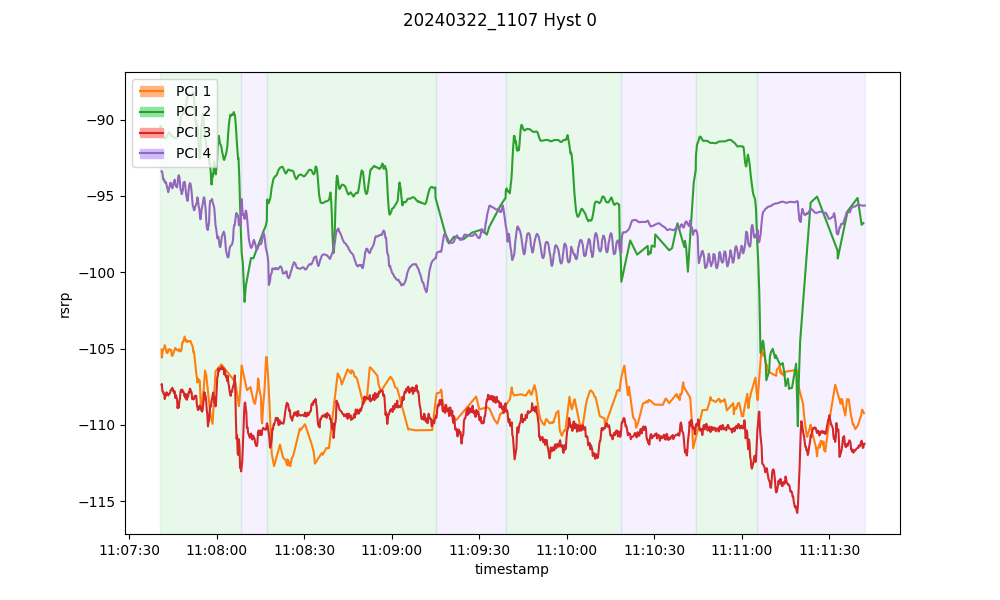
\includegraphics[width=0.6\linewidth]{src//img/5hyst0.png}
        \caption{Hysteresis Threshold: 0dBm}
        \label{fig:methods:hyst0}
    \end{subfigure}
    
    \begin{subfigure}{.9\linewidth}
        \centering
        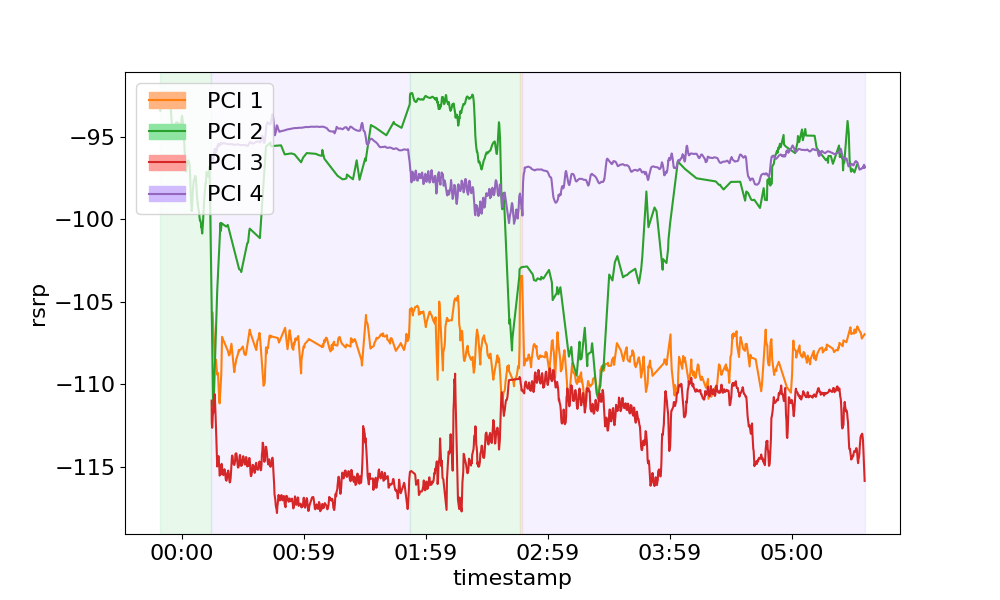
\includegraphics[width=0.6\linewidth]{src//img/5hyst3.png}
        \caption{Hysteresis Threshold: +3dBm}
        \label{fig:methods:hyst3}
    \end{subfigure}
    
    \begin{subfigure}{\linewidth}
        \centering
        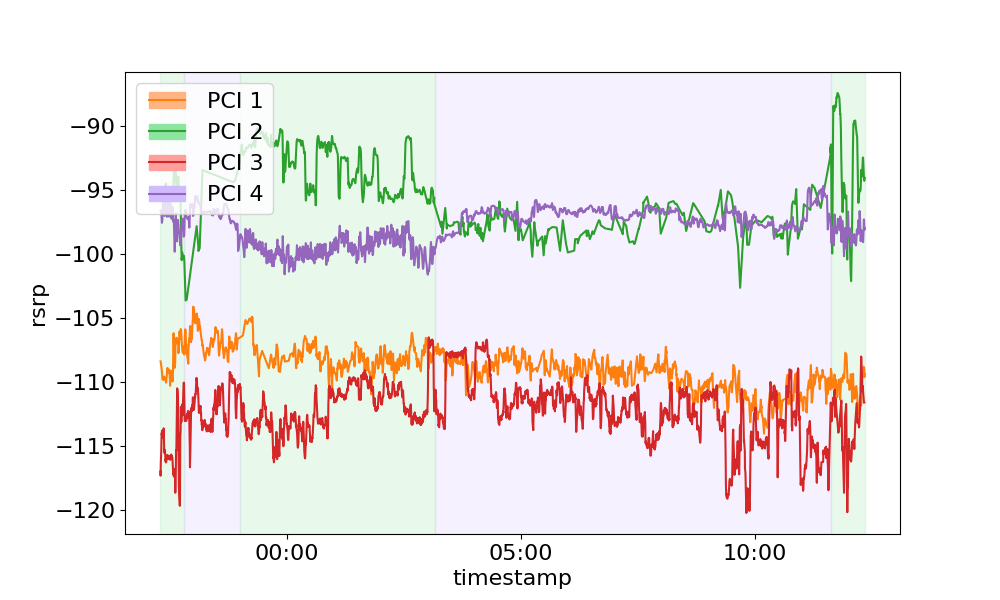
\includegraphics[width=0.6\linewidth]{src//img/5hyst6.png}
        \caption{Hysteresis Threshold: +6dBm}
        \label{fig:methods:hyst6}
    \end{subfigure}
    
    \begin{subfigure}{\linewidth}
        \centering
        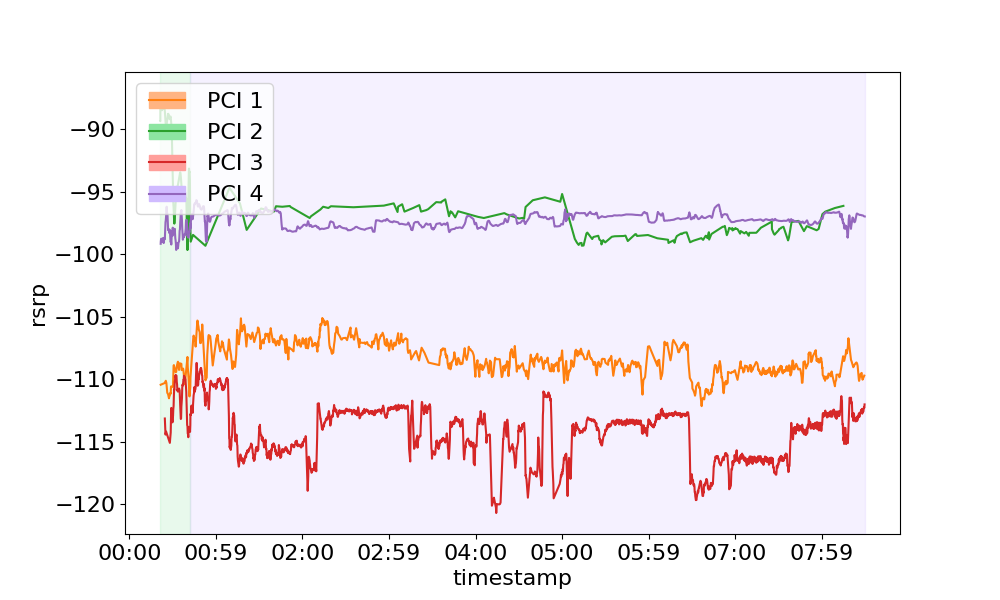
\includegraphics[width=0.6\linewidth]{src//img/5hyst9.png}
        \caption{Hysteresis Threshold: +9dBm}
        \label{fig:methods:hyst9}
    \end{subfigure}
\end{figure}

\subsubsection{Immediate Discussion}
We can conclude that choosing a higher hysteresis value greatly reduces the handover rate.

\chapter{Synthesis of Findings}
\tocomplete{Write Synthesis of Findings}

\chapter{Future Directions}
\tocomplete{Write Future Directions}

\chapter{Conclusions}
\tocomplete{Write Conclusions}

\listoftodos

\bibliographystyle{abbrvnat}

% \bibliographystyle{plain}
\bibliography{references}


% You may delete everything from \appendix up to \end{document} if you don't need it.
\appendix

\include{src/appendix_A}


\end{document}

%%%%%%%%%%%%%%%%%%% NOTES %%%%%%%%%%%%%%%%%%%%%%%%%
You can use the following rough page count estimate to distribute content across a 40-page dissertation while ensuring each section is adequately addressed. This distribution considers the typical depth and detail required for each section in a comprehensive study like yours on "Understanding 5G Handover through Machine Learning and Signal Processing."

[2] Introduction (3-4 pages): Introduce the topic and outline the study's research gap, objectives, and significance. Given the topic's complexity, enough space is needed to set the stage for your research.

[6(5.3)] Background (5-6 pages): Provide a detailed literature review and theoretical framework for 5G, handover processes, machine learning, and signal processing. This section establishes the foundation for your research.

[5(4.2)] Exploratory Research Design (5-6 pages): Describe the methodology in detail, including the design of your exploratory research, the selection of machine learning models, data collection methods, and the rationale behind your choices. This section must be thorough to ensure the validity and reliability of your research.

[8(7)] Experimentation (10-12 pages): Detail the experimental setup, the implementation of machine learning techniques, the processing of signal data, and the analysis performed. Given that this is the core of your research, it should be the most detailed, comprehensively documenting your experiments and initial findings.

[1(0)] Synthesis of Findings (6-7 pages): Present the results of your experiments, interpret the data, and discuss how your findings address the research questions or hypotheses. This section synthesizes the data collected with the literature reviewed to draw meaningful conclusions about indoor handover processes.

[1(0)] Future Directions (3-4 pages): Based on your findings, suggest areas for future research, potential improvements in technology or methodology, and how your work could be expanded or applied in other contexts. This section highlights the significance of your work and its implications for future studies.

[1(0)] Conclusions (2-3 pages): Summarize the key findings of your research, its limitations, and the practical implications for 5G network development and optimization. This section concisely encapsulates the essence and impact of your study.